\chapter{Reflection and outlook}

The reflection chapter concludes the second steps in the epic quest of the academic team towards the improvement of data quality and data availability at Swiss Post. It evaluates the project with regard to methodology, content, and personal learnings, and then concludes with an outlook on how the project may be followed up.

\begin{figure}[H]
    \centering
    
\includegraphics[width=0.8\textwidth]{./content/img/ProjectManagement/LordsOfDQM.png}
    \caption{Reflections with the lords of DQM}
    \label{fig:reflection_lords_of_dqm}
\end{figure}



\section{Methodological Reflection}
In this section, the methodology is reflected. This is not limited to the project management methodology but looks overall at all methods applied.

\subsection*{What went well}
The following list of items went well, including a reasoning why they went well.

\begin{itemize}
    \item \textbf{Documentation using Miro}: The documentation of the project on Miro went well. The tool proved very useful for fast notes, which were brought into the document later. It was also used for project management and is a key information resource for the entire project.
    \item \textbf{Weekly meetings, Jour Fixe}: The Jour Fixe, as documented in Miro, was held weekly. It proved to be a valuable exchange and helped guide the work and larger tasks. Its documentation on paper was uploaded to Miro, which helped in keeping track of discussed and important decisions.
    \item \textbf{Weekly meeting structure}: The meeting structure, starting with an introduction to the topic, the deliverables worked on, and a milestone status update, helped to structure the meetings and eased the start into another session after one week. Furthermore, the predefined questions helped to keep the discussion focused on the important topics. The deliverables graphic, together with the broad description of discharged and submitted items on Miro, supported this.
    \item \textbf{Milestone structuring}: The milestones helped to keep the time effort per chapter structured. They helped to stop basic research at the right moment and to move towards the solution landscape and implementation.
    \item \textbf{Writing mode}: The writing mode, with corrections using ChatGPT based on a defined prompt, went well after it was defined. It helped to iron out earlier occurrences of non-academic writing and grammatical issues.
    \item \textbf{Kanban}: The Kanban board helped to keep track of tasks. While the usage can still be improved, noting important decisions as tasks helped to keep track of them.
\end{itemize}


\subsection*{What did not go well}

\begin{itemize}
    \item \textbf{Work on every Friday and Wednesday afternoon}: According to planning at the start of the project, the full friday with approximately eight hours and the wednesday afternoon with aproximately 4 hours at work were reserved for work on the projet. This was not always possible as the timetracking for work shows. This was compensated with working on other days then planned. However time blockers will need to be re-negotiated for the next project.
    \item \textbf{Split between work at Swiss Post and academic work}: The 50\% to 50\% split between both engagements was not possible. At the beginning of the project, a delayed work project consumed all efforts and blocked from an early start into the project tasks, while later interruptions on production systems had to be fixed imediately rather than on the next day. This affected the start of the academic project which was postponed till early October which affected the scope.
    \item \textbf{Writing speed}: The writing speed proofed to be lower than expected. Instead of reaching a first draft before Xmas holidays, the first complete draft was only available early january. This showed the need for an earlier start with more writing. 
    \item \textbf{Rewriting of chapters}: Some chapters such as the results chapter were written in a first draft which had to be completely rewritten. This was a learning regarding required academic writing structure. In the following projects, this will be known an can be evaded.
\end{itemize}



\section{Content-related Learnings}
% Was habe ich über DQM, DA, Lineage, Organisation gelernt?

\begin{itemize}
    \item \textbf{Data lineage and reporting pipeline}: The complex data lineage at Swiss Post, including the path from physical sensors through Apache Kafka to Amazon S3 storage. The number of steps until the data is available as a report is higher than expected. Even before the data is stored in the cloud in a raw state, it has already passed through at least three processing steps. Adding the reporting pipeline further increases the complexity, which at this stage is at least partly the responsibility of the reporting team.
    \item \textbf{Where to check data quality and availability}: Data quality and availability checks need to be set up at different positions within the data lineage and reporting pipeline. While data availability is best checked early, data quality can only be checked in later stages when the data is joined with organisational information. For example, checking whether a postal code is valid requires a join with a postal code register when not only the number of digits but whether the code exists should be verified.
    \item \textbf{Independence of data quality and availability}: Data can be available but incorrect, or unavailable but correct. This is because availability can be time-based. For example, data needs to be available at 07:00; if it is not available at 07:00 but arrives at 07:02 and is correct, the data was simultaneously unavailable while its quality was acceptable.
    \item \textbf{Technical documentation requirements}: When setting up the documentation for the DQM team, it became apparent which information is important, such as missing account information in the first version. Documentation within the same team often does not require such details, but communication with another team requires this key information, including more guidance on how to navigate an unfamiliar environment, such as the different databases in Amazon Athena.
    \item \textbf{Use case feasibility}: The research and documentation of existing checks performed by the business showed that they can be replaced with automated rule-based checks. Furthermore, the implementation demonstrated the steps required to set up the rules for future DQM checks.
    \item \textbf{Tool-related}: During the work, many new tools were explored, such as DSP with its data lineage capabilities. This enabled the acquisition of new knowledge that is useful for future work.
    \item \textbf{Language-related}: The analysis of the query structure used in the DQM view helped to understand Amazon Athena–specific structures and also deepened knowledge of CTE usage in three-layered aggregations.
    \item \textbf{Usefulness of heterogeneity}: While the heterogeneity of Swiss Post poses challenges at the reporting level, it is essential at the operational and risk management levels. For example, managing plants of different sizes in the same way would create management overhead, and relying on a single hardware provider would introduce significant risks.
    \item \textbf{IT complexity}: Swiss Post has a large IT infrastructure that is managed by multiple teams working together towards the common goal of keeping systems running and improving them. This creates constraints, as multiple teams work on shared initiatives. While this can be beneficial, as not everything needs to be handled by a single team, it also requires coordination of solutions and architectures, often shifting new implementations from greenfield to brownfield environments.
\end{itemize}



\section{Personal Learnings \& Outlook}

In the course of this work, the author has learned many things; the following list summarises the most important learnings and their expected impact on future work.

\begin{itemize}
    \item \textbf{Importance of better planning}: Instead of assuming that something may be done in two or three days, the amount of learning required for unknown tools must be considered. Tasks should therefore be evaluated with regard to the tooling required. If the tooling is unknown, the learning time should be added to the time required for the task.
    \item \textbf{Organisational constraints}: Due to the size of Swiss Post, many activities happen in parallel. Multiple teams can work on the same initiatives, but often on different aspects. Identifying these activities prior to starting can help to avoid duplicated research. This, however, requires more preparation time and management, as well as communication within the organisation.
    \item \textbf{Research the obvious earlier}: For example, the DQM team did have some documentation, but this documentation was not sufficient for the rule-based DQM initiative. Reviewing this information in more detail earlier in the project would lead to a better understanding of the initial situation.
    \item \textbf{Communication with external teams}: External teams have different delivery goals and timelines. To avoid incorrect assumptions about their deliverables, these plans need to be tracked explicitly. This requires earlier communication and research into their timelines and delivery goals. Based on this information, the planning of the project team can be adapted.
    \item \textbf{Start the writing earlier}: The writing process was started early with the first chapters; however, the bulk of the writing was completed after the implementation. Starting the writing process earlier would shift research activities that occur during writing to an earlier stage. Having the chapters on which the implementation is based available earlier also allows the work to be structured more effectively.
    \item \textbf{Focus on what is relevant}: When taking screenshots, it is not necessary to capture the entire screen. It is more important to highlight the relevant information rather than documenting where in the tool the information can be found. Using lenses or smaller screenshots is therefore identified as a learning and goal for the next project.
\end{itemize}




\section{General setup, next steps}
\section{Todo, rewrite this... taken from Reseach Chapter}
As stated earlier the solutional goal of this project and its follow up is to provide an MVP for DQM, from
which the key learnings will enable the full “future state” reporting solution. This MVP should implement
anautomaticdataqualitycheck,replacinganoccasional,nonautomatedcheckperformedbythebusiness.
This is important, as the DQM check is currently executed by the business instead of IT, which creates
challenges with regard to the desired target state. The expected situation would be that IT executes data
quality checks and de nes thresholds together with the business. At present, however, the knowledge
about thresholds and other relevant information resides solely with the business.
Insummary,havingITrunthedatacheckswouldenablecontinuousfollow-upofdataquality. Forexample,
a report based on automatically executed checks could show system uptime over a longer period of time.
This information would later allow IT to extrapolate standard value ranges, which in turn would enable
the de nition of alerting thresholds. In short, having DQM checks executed automatically rather than
occasionally by the business provides multiple bene ts for both IT and the business

Here... the planning of the master thesis was a big part of all the follow up work

\begin{figure}[H]
    \centering
    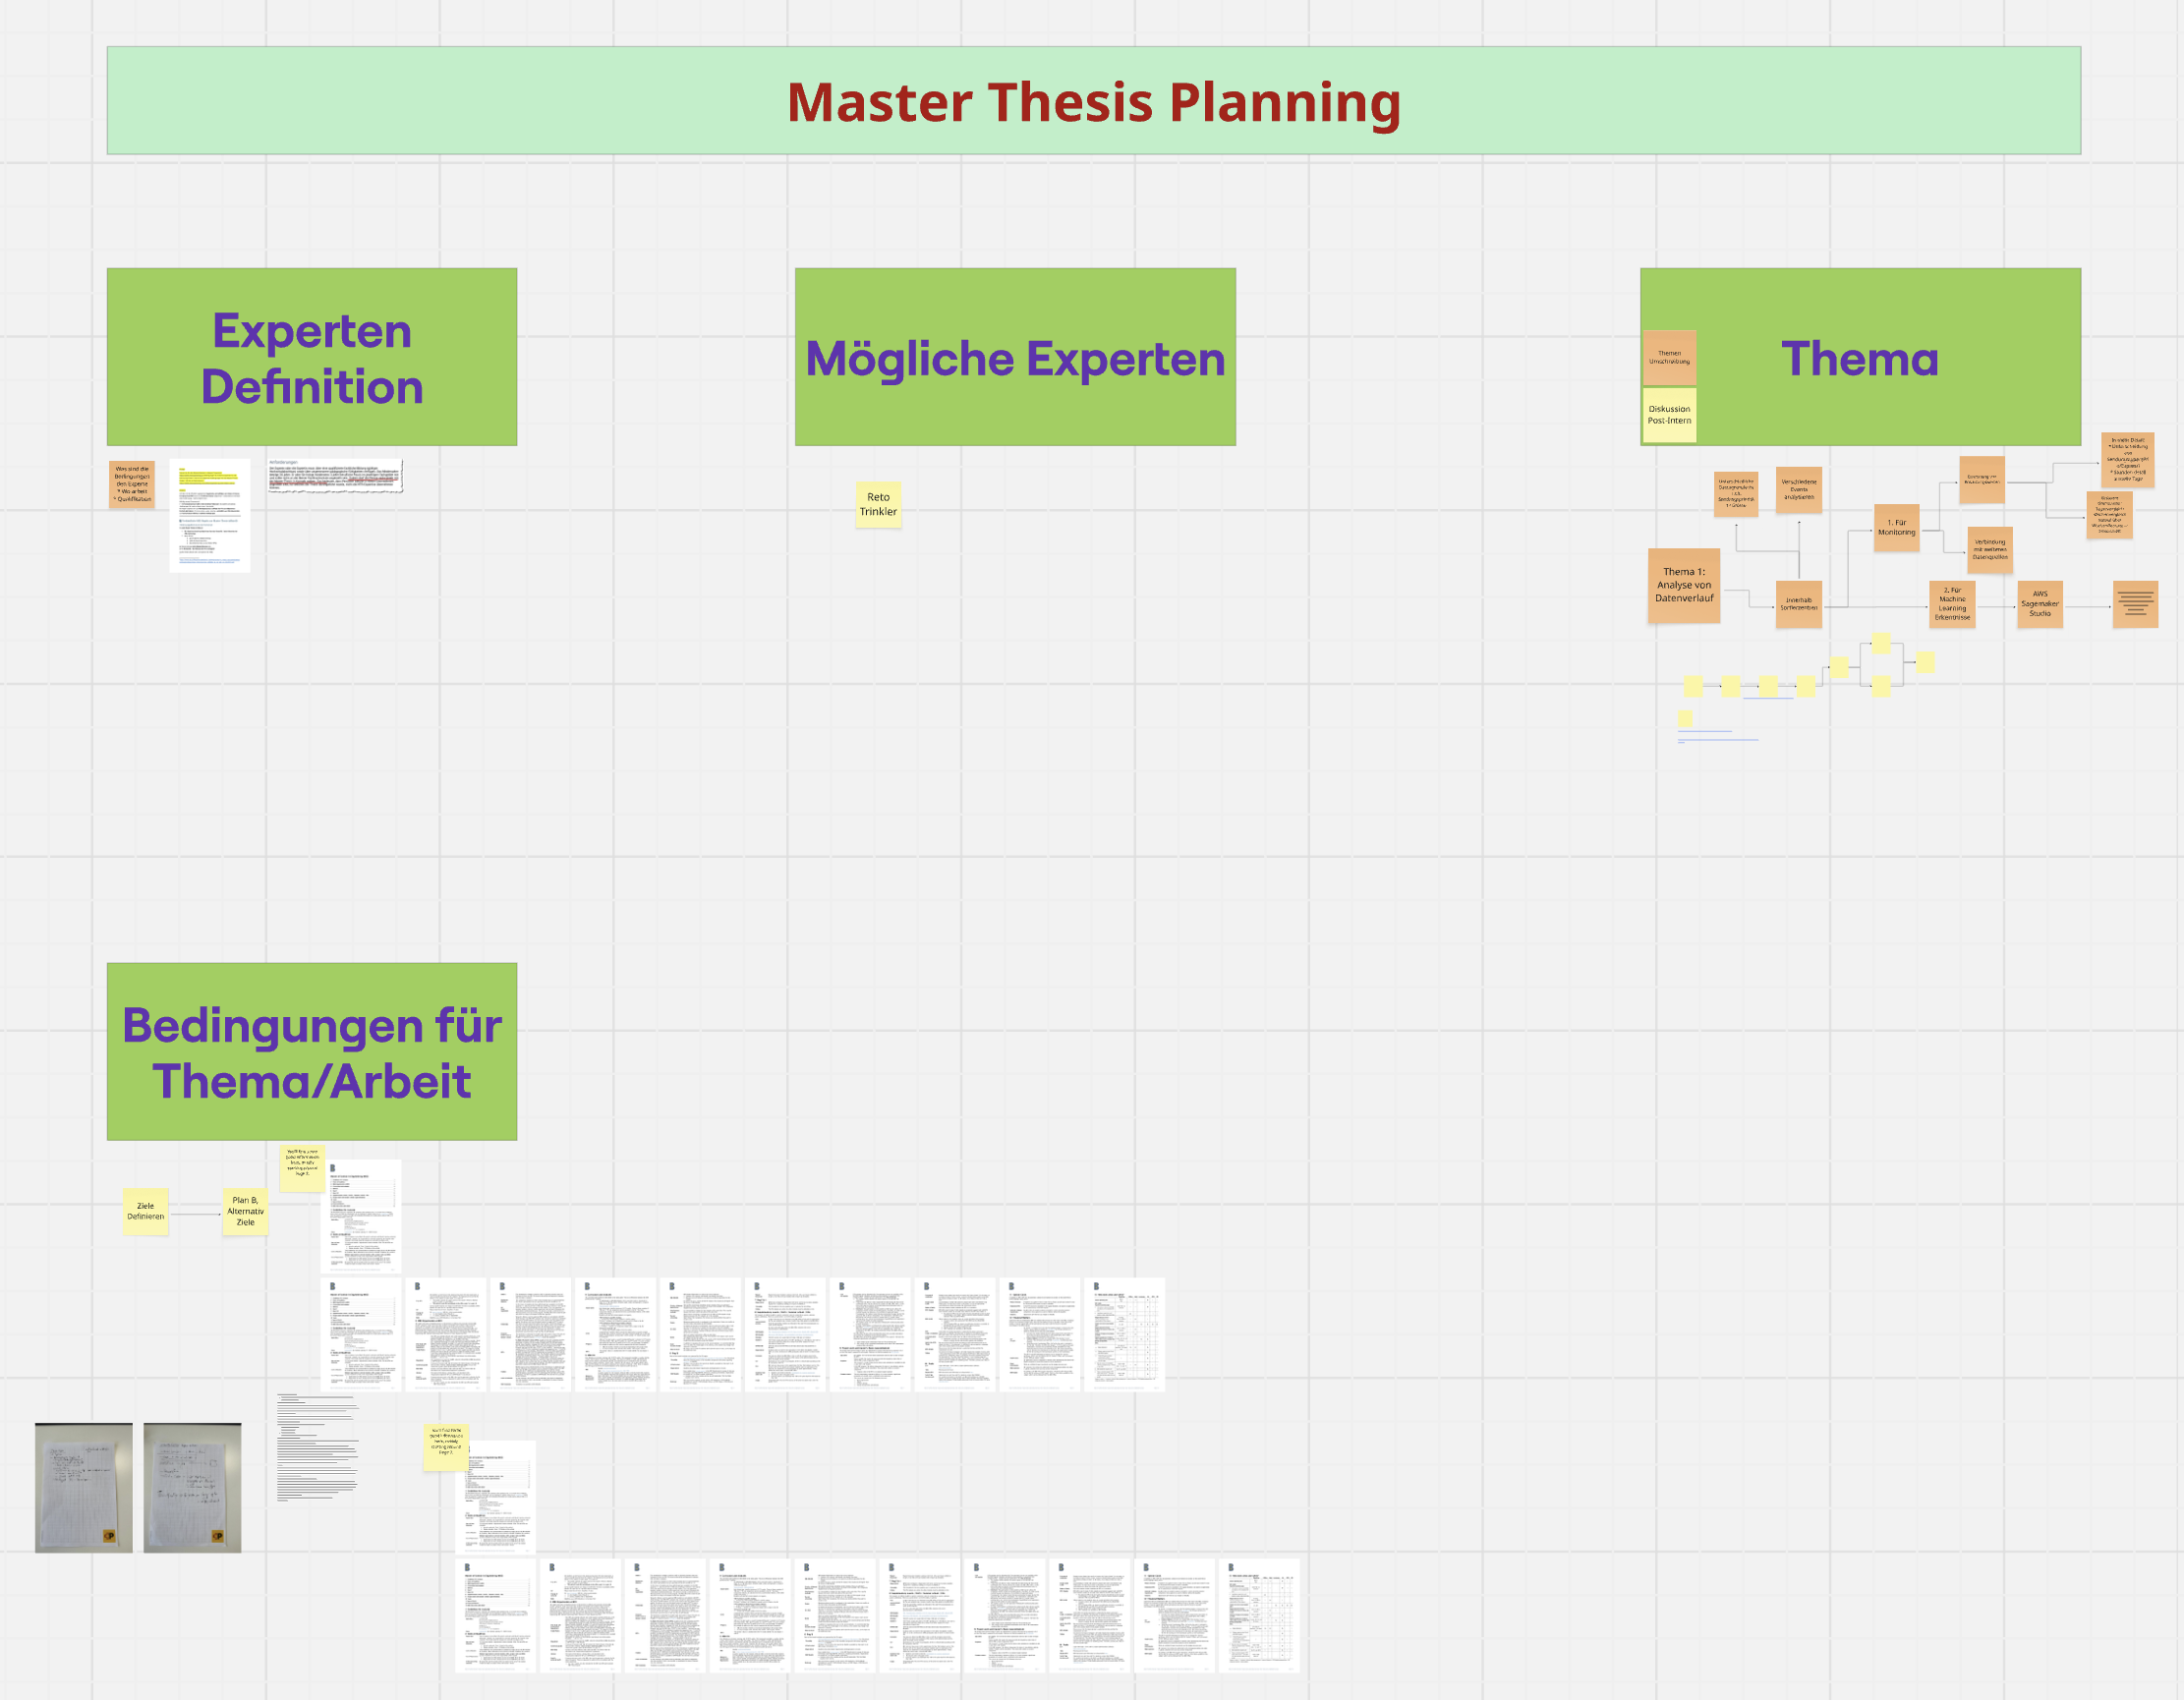
\includegraphics[width=\textwidth]{./content/img/MiroBoard_MasterThesis_Planning.png}
    \caption{Extract of the Miro board illustrating the planning of the subsequent master's thesis. The section documents initial ideas, work packages, dependencies and planning considerations that emerged during Project~2 and served as preparation for the continuation of the research.}
    \label{fig:annex_miro_masterthesis}
\end{figure}